\documentclass[10pt,a4paper,oneside]{article}

%-----------------------------------------------------------------------
% Packages
\usepackage[utf8]{inputenc}
\usepackage[italian]{babel}
\usepackage{amsmath}
\usepackage{amsfonts}
\usepackage{amssymb}
\usepackage{graphicx}
\usepackage{tabularx}
\usepackage{booktabs}
\usepackage{multirow}
\usepackage{lmodern}
\usepackage[colorlinks]{hyperref}

%-----------------------------------------------------------------------
% Package configuration
\hypersetup{
 urlcolor = blue
}

%-----------------------------------------------------------------------
% Heading
\title{Specifica Progetto di Laboratorio}
\author{Programmazione ad Oggetti}
\date{a.a. 2024/25}

%-----------------------------------------------------------------------
% Document
\begin{document}
\maketitle

%-----------------------------------------------------------------------
\section{Introduzione}
L'obiettivo del progetto è sviluppare un sistema di gestione per una biblioteca che supporti diversi tipi di media, come libri, film e articoli di riviste, utilizzando il linguaggio di programmazione C++ e il framework \href{https://www.qt.io/?hsLang=en}{Qt} per la creazione di un'interfaccia grafica utente (GUI). L'applicazione deve permettere agli utenti di gestire la collezione multimediale, ovvero aggiungere, modificare e rimuovere media esistenti, nonché visualizzare le informazioni di ciascun tipo di media in un'interfaccia chiara e intuitiva.

Ogni tipo di media sarà rappresentato da una classe derivata da una classe base comune. Gli utenti dell'applicazione dovranno essere in grado di cercare, creare, visualizzare, modificare e cancellare i media, interagendo con i loro attributi specifici, come ad esempio l'autore, l'anno di pubblicazione, o il regista.

Il progetto potrà essere sviluppato da un \textbf{singolo studente} oppure da una \textbf{coppia di studenti} e dovrà richiedere \textbf{approssimativamente 40 ore di lavoro} complessivo individuale.

La GUI potrà ispirarsi liberamente sia ad applicazioni desktop che a sistemi mobile. È possibile adottare pattern architetturali come il \emph{Model-View-Controller} o \emph{Model-View} per la progettazione della GUI. Il framework Qt offre una documentazione completa e dettagliata che sarà la principale guida di riferimento per lo sviluppo dell'interfaccia grafica. Si incoraggia anche l'applicazione di design pattern comunemente utilizzati in C++ per migliorare la manutenibilità e l'estensibilità del progetto.

La valutazione del progetto e il voto dell'esame scritto saranno calcolati separatamente ed entrambi concorreranno al voto finale dell'esame. In linea generale, il voto dell'esame scritto avrà un peso maggiore, ma la valutazione del progetto potrà influire positivamente o negativamente sul risultato finale. Gli studenti avranno la possibilità di ripresentare il progetto mantenendo il voto dell'esame scritto, e viceversa. Tuttavia, la valutazione del progetto sarà effettuata solo per gli studenti che abbiano superato l'esame scritto e si siano iscritti correttamente nella lista Uniweb per la registrazione del voto finale.



%-----------------------------------------------------------------------
\section{Vincoli}
Il progetto deve obbligatoriamente soddisfare i seguenti vincoli:
\begin{enumerate}
 \item essere un \textbf{lavoro originale} dello studente o della coppia di studenti
 \item essere interamente \textbf{scritto in C++}
 \item prevedere un'\textbf{interfaccia grafica} realizzata in Qt
 \item \textbf{compilare senza errori} sulla macchina virtuale fornita (sono tollerati, sebbene generalmente penalizzati, i \emph{warning} durante la compilazione)
 \item rispettare i principi di \textbf{incapsulamento} e \textbf{\emph{information hiding}} della programmazione orientata agli oggetti: una classe deve rappresentare un singolo concetto e includere attributi e metodi con livelli di visibilità appropriati
 \item mantenere una \textbf{separazione netta} tra il modello logico e l'interfaccia grafica, ovvero il codice del modello deve essere riutilizzabile senza dipendenze dall'interfaccia; è consentito che il modello utilizzi strumenti Qt non legati all'interfaccia, come le funzioni di I/O o le classi per la gestione di JSON
 \item eseguire in maniera \textbf{efficiente e robusta}, senza errori a \emph{runtime}
 \item utilizzare il \textbf{polimorfismo in maniera non banale}; esempi di utilizzo \emph{banale} sono distruttori virtuali o semplici \emph{getter}. Un utilizzo \emph{non banale} include metodi che si comportano in maniera profondamente diversa in base al tipo dinamico dell'oggetto invocante, come la visualizzazione di interfacce o azioni specifiche per ogni tipo di media; si incoraggia l'utilizzo di uno o più \emph{design pattern}, in quanto questi richiedono spesso un uso approfondito del polimorfismo
 \item \textbf{non utilizzare metodi virtuali come \emph{getType}} che restituiscono una stringa rappresentate il tipo dell'oggetto per gestire il controllo di flusso in sostituzione al polimorfismo; l'uso di tali metodi è consentito unicamente se finalizzati a mostrare effettivamente una semplice stringa
 \item implementare una \textbf{gerarchia di classi} per i media con almeno \textbf{tre classi concrete} (ad esempio per libri, film e articoli) per i progetti svolti singolarmente, o almeno \textbf{cinque classi concrete} per i progetti svolti in coppia; in ogni caso le classi dovranno presentare differenze significative, quali attributi e metodi diversi
 \item consentire la \textbf{creazione, ricerca, modifica e cancellazione} di media tramite l'interfaccia grafica; le procedure di creazione e modifica, in particolare, devono tenere conto dei differenti attributi delle classi concrete
 \item implementare la \textbf{persistenza dei dati} per i media in un file locale in almeno \textbf{un formato strutturato} (ad esempio JSON o XML) per i progetti di individuali, o in almeno \textbf{due formati strutturati} per i progetti di coppia
 \item consentire il \textbf{salvataggio e il caricamento} dei file contenenti i dati dei media attraverso finestre di dialogo grafiche, evitando percorsi cablati nel codice sorgente
 \item gestire la \textbf{navigazione tra le diverse schermate} all'interno della stessa finestra, evitando l'apertura non necessaria di molteplici finestre; fanno eccezione finestre di dialogo quali la selezione dei file, modali ed eventuali popup di conferma
 \item essere corredato di una \textbf{relazione} in formato PDF, in lingua italiana o inglese, di massimo 8 pagine con testo a 10pt, che riporti:
 \begin{enumerate}
  \item nome, cognome e numero di matricola di tutti i componenti del gruppo (o del singolo autore)
  \item una breve introduzione che descriva il contesto del progetto
  \item la descrizione delle classi principali del modello logico
  \item la descrizione dell'utilizzo non banale del polimorfismo, identificando quali metodi sono polimorfi (in maniera "non banale") e qual è il loro valore aggiunto all'interno del progetto
  \item la descrizione del metodo di persistenza dei dati
  \item la descrizione delle funzionalità aggiuntive implementate
  \item la rendicontazione delle ore previste e di quelle effettivamente svolte
  \item solo per i progetti svolti in coppia: la suddivisione delle attività tra i membri del gruppo
  \item solo per progetti riconsegnati: una sezione che riporti le modifiche rispetto all'ultima consegna
 \end{enumerate}
 In caso di progetto di coppia, \textbf{le relazioni devono essere distinte}. Assieme alle specifiche viene fornito un modello commentato di relazione, il cui utilizzo non è obbligatorio. Si suggerisce l'uso di \href{https://it.wikipedia.org/wiki/LaTeX}{LaTeX} per redigere la relazione, dato che è largamente utilizzato in ambito accademico
\end{enumerate}

La Fig.~\ref{fig:skeleton} mostra un esempio di struttura dell'interfaccia grafica.

\begin{figure}[t]
	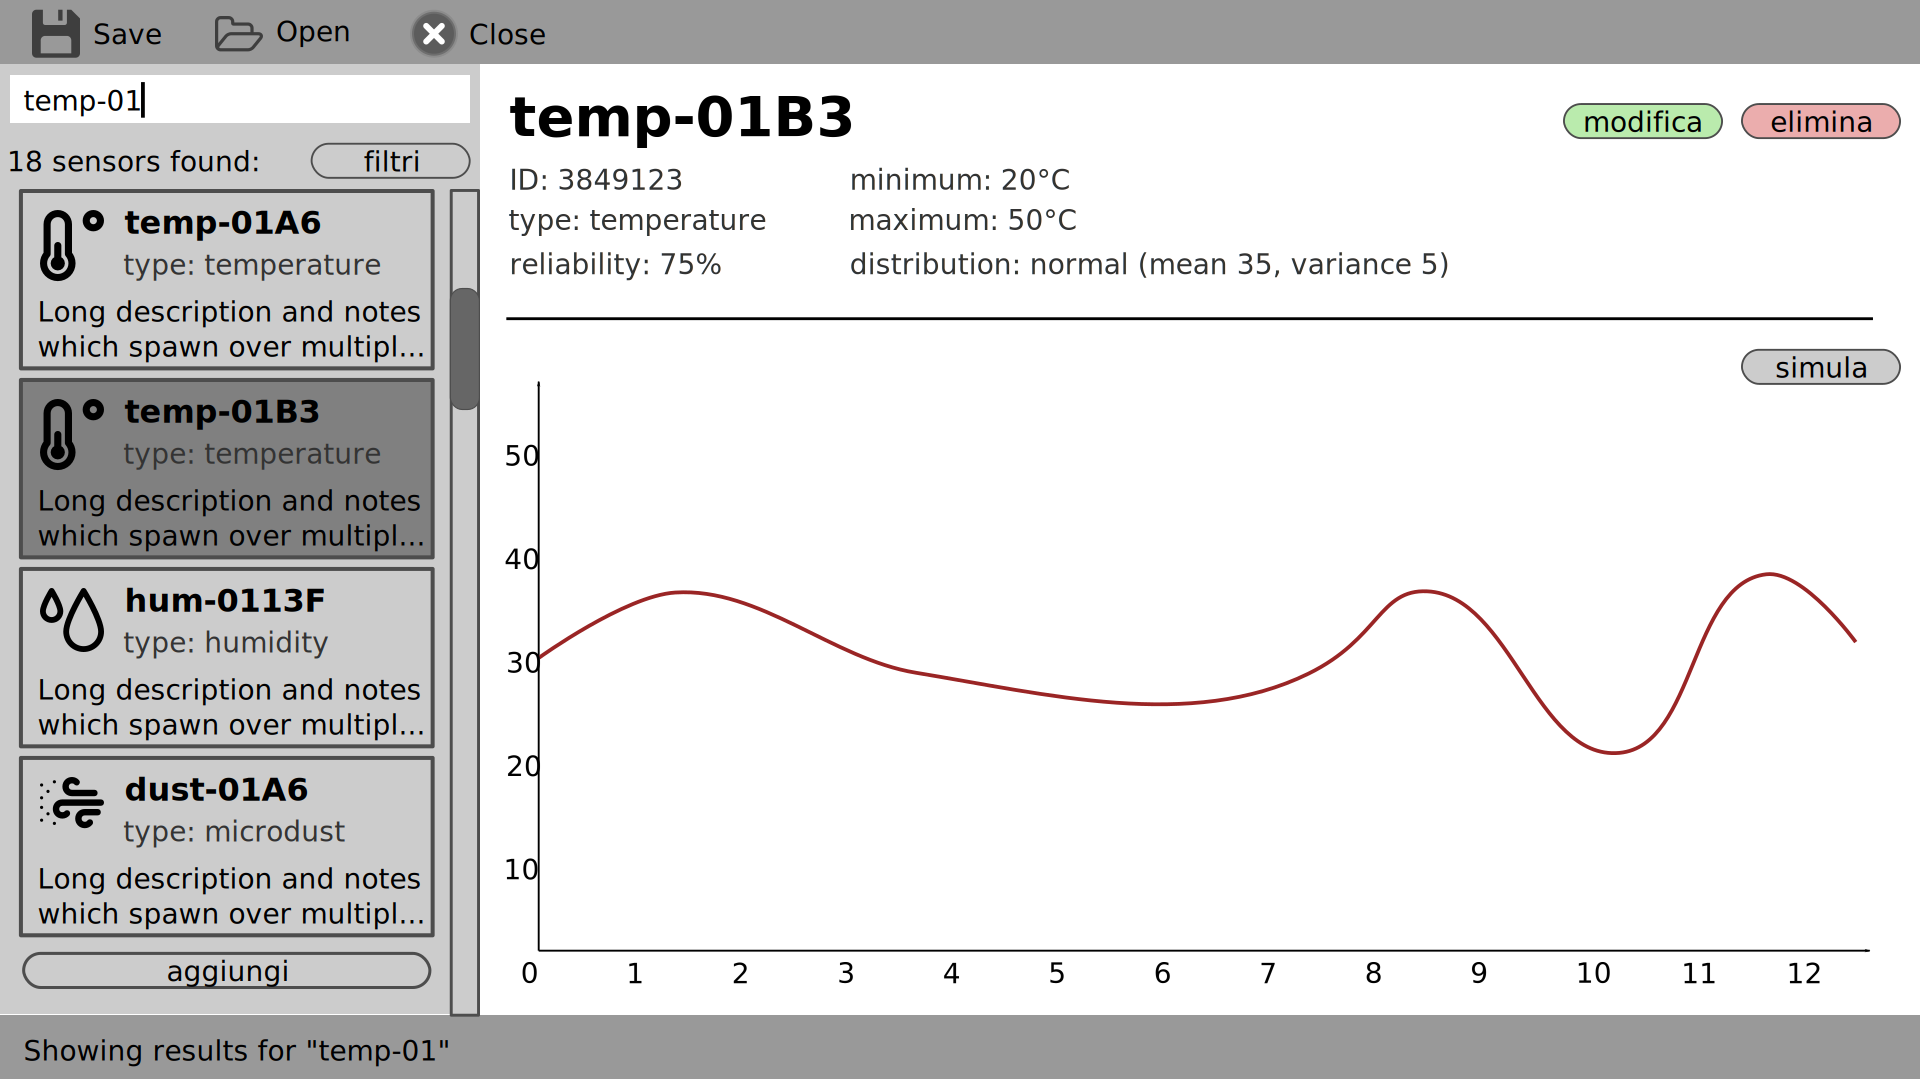
\includegraphics[width=0.95\textwidth]{assets/gui-skeleton-sample}
	\caption{Esempio di scheletro di una possibile interfaccia della finestra principale}\label{fig:skeleton}
\end{figure}

%-----------------------------------------------------------------------
\section{Consegna}
La consegna avverrà tramite il Moodle del corso, all'interno del quale saranno attivate cinque sessioni di consegna del progetto per gli altrettanti appelli d'esame previsti durante l'anno accademico (due sessioni di consegna a gennaio/febbraio 2025, due sessioni di consegna a giugno/luglio 2025, 
una sessione di consegna a settembre 2025). Si dovrà consegnare un unico archivio in formato zip della dimensione massima di 256MB attraverso l'apposita pagina Moodle. \textbf{Non saranno accettati tentativi di consegna con modalità diverse o formati che non siano zip}. La cartella compressa dovrà contenere:
\begin{itemize}
 \item la relazione in formato PDF
 \item una sottocartella con i file sorgente del progetto (.h, .cpp, .pro, eventuali sottocartelle) ed eventuali file multimediali necessari (immagini, icone, ecc.)
 \item almeno un file d'esempio per la persistenza dei dati (almeno due, in diversi formati, per i progetti in coppia)
\end{itemize}
La cartella \emph{non dovrebbe} contenere codice oggetto compilato, eseguibili, file generati dall'IDE o in generale qualsiasi file non utile ai fini della valutazione. Si raccomanda di verificare il corretto caricamento dei file su Moodle e di comunicare tempestivamente eventuali malfunzionamenti.

Nei progetti di coppia ogni studente dovrà provvedere separatamente alla propria consegna includendo il codice (lo stesso per i due membri della coppia) e la propria relazione (diversa per ciascuno). Se nella coppia solamente uno studente è sufficiente all'esame scritto, questo studente può comunque procedere alla consegna del progetto con l'obiettivo di finalizzare l'esame. Si ricorda che la valutazione del progetto con relativo \emph{feedback} avverrà solamente per gli studenti sufficienti all'esame scritto ed iscritti alla lista uniweb per il voto finale.


%-----------------------------------------------------------------------
\section{Criteri di valutazione}
Il progetto viene valutato sulla base dei vincoli obbligatori e delle funzionalità implementate. Più precisamente, \textbf{se uno o più vincoli obbligatori non risultano soddisfatti il progetto verrà considerato insufficiente} e sarà necessaria una riconsegna in uno degli appelli successivi. Viceversa, \textbf{se tutti i vincoli obbligatori sono soddisfatti il progetto è considerato (almeno) sufficiente} e la valutazione aumenterà in base alla qualità delle funzionalità sviluppate e, in misura minore, in base alla qualità della relazione.

Una funzionalità viene valutata positivamente in base alla sua pertinenza al tema, all'utilità, all'usabilità, alla complessità e alla qualità del codice attraverso cui è implementata. Funzionalità più semplici o generiche migliorano la valutazione, sebbene non tanto quanto idee più complesse o articolate. Le scorciatoie da tastiera, per esempio, sono migliorie generiche semplici da ottenere con poche righe di codice in Qt, così come la gestione del ridimensionamento delle finestre o l'uso di icone. Per contro l'integrazione con un sistema di API o l'uso di basi di dati come SQL o MongoDB per la persistenza sono significativamente più complessi e richiedono la scrittura di classi apposite.

Poiché il corso non tratta di usabilità o resa estetica della GUI la loro mancanza \textbf{non verrà penalizzata}, purché questo non pregiudichi il corretto funzionamento del programma. Tuttavia, se il progetto viene sviluppato ponendo particolare attenzione a queste caratteristiche, verrà riconosciuto un bonus come se si trattasse di una funzionalità aggiuntiva.

La valutazione terrà conto dello \textbf{storico delle valutazioni}, e vedrà una progressiva riduzione all'aumentare del numero di consegne.

La qualità della relazione, pur avendo un'incidenza minore, verrà valutata sulla base della completezza, della chiarezza e della coesione. \textbf{Errori linguistici evidenti} come sistematica mancanza di punteggiatura o errori di battitura frequenti \textbf{verranno penalizzati}. È possibile redigere la relazione in Italiano o Inglese, a propria discrezione. La scelta della lingua non avrà effetti sulla valutazione.

Ciascuna finestra di consegna presente nella pagina Moodle del corso mostrerà una data limite: \textbf{non sarà in alcun modo possibile consegnare oltre tale data o con modalità diverse da quelle previste}.

La valutazione del progetto è \textbf{valida per l'intero anno accademico} e fino a che non viene (ri)consegnato un progetto.

La valutazione è accompagnata da un \emph{feedback} testuale che motiva la valutazione ed evidenzia i punti di forza e debolezza del progetto. È possibile riconsegnare un progetto per ottenere una nuova valutazione, che potrebbe anche essere peggiorativa, tuttavia se si seguono le indicazioni fornite dal \emph{feedback} sarà generalmente migliorativa. La valutazione è \emph{idempotente}: riconsegnare lo stesso progetto senza modifiche produrrà esattamente la stessa valutazione. Se un progetto viene riconsegnato senza la sezione riportante le modifiche rispetto alla consegna precedente nella relazione, questo non verrà valutato nuovamente e riceverà automaticamente la stessa valutazione della consegna precedente.

Consegnare un progetto svolto anche parzialmente da altri (con o senza il loro consenso) oppure generato da sistemi automatici comporta automaticamente l'insufficienza.

\begin{figure}[ht]
 \centering
 \includegraphics[width=0.95\linewidth]{assets/evaluation-criteria}
 \caption{Schema di valutazione indicativo}
 \label{fig:evaluation}
\end{figure}

\iffalse
\begin{table}[ht]
 \caption{Griglia di valutazione indicativa}
 \begin{tabularx}{\linewidth}{r X r}
  \textbf{Area} & \textbf{Voce} & \textbf{Punti} \\
  \toprule
  \multirow{2}{*}{Vincoli} & Uno o più vincoli non sono soddisfatti & $-\infty$ \\
  \addlinespace
  & Tutti i vincoli sono soddisfatti       & 18 \\
		
  \midrule
  \multirow{3}{*}{OOP} & Rispetto dei principi di incapsulamento e \emph{information hiding} & 1 \\
  \addlinespace
  & Uso corretto di ereditarierà e composizione & 2 \\
  \addlinespace
  & Uso corretto e approfondito del polimorfismo               & 3 \\

  \midrule
  \multirow{4}{*}{Funzionalità} & Ricerca parziale \emph{case-insensitive} in tempo reale &   1 \\
  \addlinespace
  & Ricerca avanzata configurabile &   1 \\
  \addlinespace
  & Scorciatoie da tastiera        & 0.5 \\
  \addlinespace
  & Altre funzionalità pertinenti  & $\leq$ 3 \\

  \midrule
  \multirow{6}{*}{GUI} & Visualizzazione differenziata per tipo di dato &   1 \\
  \addlinespace
  & Corretta gestione del ridimensionamento          &   1 \\
  \addlinespace
  & Utilizzo di icone e stili grafici                &   1 \\
  \addlinespace
  & Utilizzo pertinente di immagini o altri elementi multimediali & 0.5 \\
  \addlinespace
  & Vengono considerati principi di usabilità        & 0.5 \\
  
  \midrule
  Relazione & Errori linguistici evidenti e sistematici & -1 \\
  \bottomrule
 \end{tabularx}
\label{tab:evaluation}
\end{table}
\fi

La Fig. \ref{fig:evaluation} presenta la distribuzione dei pesi assegnati alle diverse caratteristiche del progetto, da considerarsi indicativa e utile come guida nello sviluppo. Poiché la valutazione dipende dalle funzionalità scelte dagli studenti, la griglia serve principalmente come riferimento orientativo.

\section{Verbalizzazione del voto}
La registrazione del voto finale è possibile solo dopo:
\begin{itemize}
 \item avere superato con valutazione maggiore o uguale a 18 la prova scritta
 \item essersi iscritti alla lista Uniweb della per la registrazione del voto finale
 \item avere consegnato il progetto entro la scadenza prevista per la sessione in cui si intende verbalizzare il voto e aver ottenuto una valutazione positiva
\end{itemize}
Si ricorda che le liste Uniweb verificato il soddisfacimento delle propedeuticità e hanno una data di chiusura anticipata di almeno 5 giorni. Non saranno ammesse iscrizioni manuali in ritardo, per nessun motivo.

La valutazione dei progetti sarà completata generalmente entro 15 giorni dalla consegna, in base al numero di progetti da esaminare. Una volta pronta, la valutazione finale, comprensiva del voto della prova scritta e del progetto, sarà caricata su Uniweb, mentre il \emph{feedback} relativo al progetto verrà inviato tramite Moodle esclusivamente agli utenti iscritti alla lista Uniweb. In caso di valutazione negativa del progetto l'esame non sarà superato: sarà quindi necessaria la riconsegna del progetto per una successiva scadenza di consegna all'interno dello stesso anno accademico; in questo caso il voto dell'esame scritto rimane comunque valido. Lo studente che rifiuterà il voto finale proposto via Uniweb dovrà riconsegnare il progetto per una successiva scadenza di consegna nello stesso anno accademico (tranne all'ultimo appello d'esame, per cui ovviamente non esiste una successiva scadenza di consegna), cercando quindi di porre rimedio ai punti deboli segnalati nel \emph{feedback} di valutazione e descrivendo obbligatoriamente le modifiche apportate al progetto nella relazione aggiornata; anche in questo caso il voto sufficiente dell'esame scritto rimane comunque valido. 



%-----------------------------------------------------------------------
\section{Note}
La parte di laboratorio dell'insegnamento di Programmazione a Oggetti ha una propria pagina ufficiale su GitHub all'indirizzo \href{https://github.com/Unipd-Object-Oriented-Programming}{github.com/Unipd-Object-Oriented-Programming}. Questo spazio contiene il materiale didattico relativo a questo modulo dell'insegnamento, inclusi i lucidi delle lezioni e gli esempi del codice, suddivisi per anno accademico.

I video-tutorati dell'anno accademico 2020/2021 del tutor Benedetto Cosentino dedicati all'apprendimento delle caratteristiche di base del framework Qt per la progettazione di GUI sono disponibili su \href{https://www.youtube.com/playlist?list=PLH_Fd-836q-VcqWnnzsq3GOF2-0i_Az7p}{YouTube}.

\end{document}
